\section{Dataset}
\label{sec:dataset}

The dataset is called DOLOS and it is collected from the british gameshow "Would I lie to you". 
In the gameshow, two teams consisting of 6 persons try to deceive each other. 
The speaker reads a event from everyday life, that only he knows is true or false. 
Then the opposing team has to figure out if he is lying by asking him questions that he has to answer. 

Video clips from an episode had to satisfy two requirements: The participant is talking about the truth or the lie and 
can be clearly understood, without any background noise, and the face of the participant must be clearly visible.
In total, 1675 video clips were extraced, making it the largest dataset of this kind. 
Each clip was annotated manually for non-verbal deceptive cues, using the MUMIN coding sheme, which categorizes 
actions in categories shown in figure \ref{fig:Mumin}

\begin{figure}[t]
  \centering
   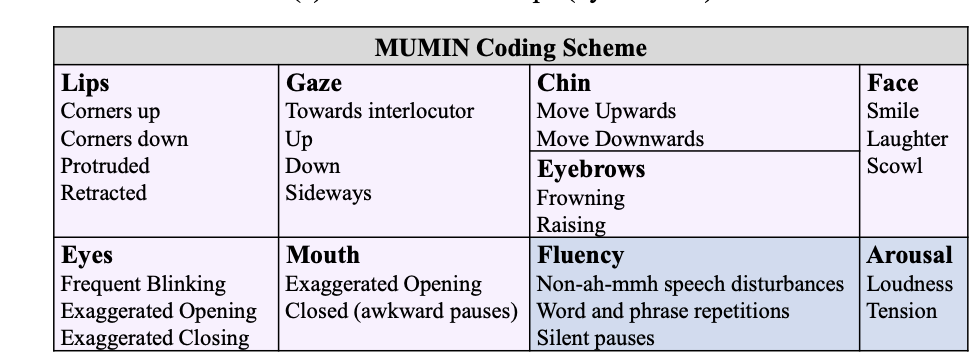
\includegraphics[width=0.8\linewidth]{images/Mumin Coding Sceme.png}
   \caption{The different categories of the MUMIN coding sheme. Visual cues are in pink and audio cues are in blue.}
   \label{fig:Mumin}
\end{figure}